\documentclass{article}
\usepackage{amsmath,amsfonts,amsthm,amssymb,amsopn,bm}
\usepackage[margin=.9in]{geometry}
\usepackage{graphicx}
\usepackage{url}
\usepackage[usenames,dvipsnames]{color}
\usepackage{fancyhdr}
\usepackage{multirow}
\usepackage{listings}
\usepackage{hyperref}

\definecolor{keywords}{RGB}{255,0,90}
\definecolor{comments}{RGB}{0,0,113}
\definecolor{red}{RGB}{160,0,0}
\definecolor{green}{RGB}{0,150,0}
 
\lstset{language=Python, 
        basicstyle=\ttfamily\tiny, 
        keywordstyle=\color{keywords},
        commentstyle=\color{comments},
        stringstyle=\color{red},
        showstringspaces=false}

\newcommand{\argmax}{\arg\!\max}
\newcommand{\argmin}{\arg\!\min}
\newcommand{\field}[1]{\mathbb{#1}}
\newcommand{\1}{\mathbf{1}}
\newcommand{\E}{\mathbb{E}} 
\renewcommand{\P}{\mathbb{P}}
\newcommand{\R}{\field{R}} % real domain
% \newcommand{\C}{\field{C}} % complex domain
\newcommand{\F}{\field{F}} % functional domain
\newcommand{\T}{^{\textrm T}} % transpose
\def\diag{\text{diag}}

%% operator in linear algebra, functional analysis
\newcommand{\inner}[2]{#1\cdot #2}
\newcommand{\norm}[1]{\left\|#1\right\|}
\newcommand{\twonorm}[1]{\|#1\|_2^2}
% operator in functios, maps such as M: domain1 --> domain 2
\newcommand{\Map}[1]{\mathcal{#1}}
\renewcommand{\theenumi}{\alph{enumi}} 


\newcommand{\Perp}{\perp \! \! \! \perp}

\newcommand\independent{\protect\mathpalette{\protect\independenT}{\perp}}
\def\independenT#1#2{\mathrel{\rlap{$#1#2$}\mkern2mu{#1#2}}}
\newcommand{\vct}[1]{\boldsymbol{#1}} % vector
\newcommand{\mat}[1]{\boldsymbol{#1}} % matrix
\newcommand{\cst}[1]{\mathsf{#1}} % constant
\newcommand{\ProbOpr}[1]{\mathbb{#1}}
\newcommand{\points}[1]{\small\textcolor{magenta}{\emph{[#1 points]}} \normalsize}
\date{{}}

\setlength\parindent{0px}

\begin{document}
\title{Homework \#1 A}
\author{\normalsize{Spring 2020, CSE 446/546: Machine Learning}\\
\normalsize{Dino Bektesevic}}
\maketitle

Collaborated: Conor Sayers, Joachim Moeyenes, Jessica Birky, Leah Fulmer

\section*{Short Answer and “True or False” Conceptual questions}
A.0 The answers to these questions should be answerable without referring to external materials.
\begin{enumerate}
    \item \points{2} In your own words, describe what bias and variance are? What is bias-variance tradeoff? \newline
    Bias is the error we incur by assuming a model. Since models don't necessarily describe the underlying truth they will attempt to "rephrase" it in terms of assumptions and/or approximations made in the model itself. Variance is the error that comes about due to the spread in our data. At a fine enough level all processes will have some amount of variance. Fitting a model to that data will produce an estimator of recorded data set. Remeasuring and refitting a model might produce a slightly, or significantly, different estimator due to the variance between data points of the two respective data sets. That slight difference in expected estimator is the model variance. \newline
    The more complex the model we use, the more of intricate details of the underlying truth it can capture. This leads to low bias but also, if the data varies a lot between measurements, opens the doors to high variance. Having a simple model might reduce the complexity, and might be better at ignoring the variance in the data, but once fitted might not correspond with the truth. The inability to chose arbitrarily complex model without having the variance explode or, vice-versa choosing arbitrarily simple model while not having bias explode, is called bias-variance trade-off.

    \item \points{2} What happens to bias and variance when the model complexity increases/decreases? \newline
    Bias tends to reduce with model complexity while variance tends to increase. 

    \item\points{1} True or False:  The bias of a model increases as the amount of training data available increases.\newline
    False. Bias is related to underlying inability of a model to describe the truth. That statement holds irregardless of the amount of data we have. The fit gets better because the more data we train on the more variance will reduce.

    \item\points{1} True  or  False:  The  variance  of  a  model  decreases  as  the  amount  of  training  data  available increases.\newline
    True. See above, variance decreases.

    \item\points{1} True or False:  A learning algorithm will generalize better if we use less features to represent our data.\newline
    True. While true that a 1 parameter model can be great at, f.e., predicting averages of anything, they can also be useless if they can't inform us. Generally the best case scenario is when features can be identified as real parameters of an analytical model. Sometimes, for complex systems that have no good analytical model, adding more features might help, by capturing the parameters missing from the model, but in general adding more features tends to hurt the model.

    \item\points{2} To get better generalization, should we use the train set or the test set to tune our hyperparameters?\newline
    Always generalize on the train set. Hyperparameters should be tuned on the train set as well. Always work only on the train set, or potentially validation set, until the point you need to measure the true error. That is the only point at which we should use test set. 

    \item\points{1} True or False:  The training error of a function on the training set provides an overestimate of the true error of that function. \newline
    False. Training error will always be less than the test error. True error is estimated on test data set, not on the training data set.
\end{enumerate}





\newpage
\section*{Maximum Likelihood Estimation (MLE)}

A.1.  You’re a Reign FC fan, and the team is five games into its 2018 season. The number of goals scored by the team in each game so far are: $[2,0,1,1,2]$. Let’s call these scores $x_1,...,x5$.  Based on your (assumed iid) data, you’d like to build a model to understand how many goals the Reign are likely to score in their next game. You decide to model the number of goals scored per game using a Poisson  distribution. The Poisson distribution with parameter $\lambda$ assigns every non-negative integer $x=0,1,2,...$ a probability given by

$$P(x|\lambda)=\frac{\lambda^x}{x!}e^{-\lambda}$$

So, for example, if $\lambda=1.5$, then the probability that the Reign score 2 goals in their next game is $e^{-1.5}\cdot1.522!\approx0.25$. To check your understanding of the Poisson, make sure you have a sense of whether raising $\lambda$ will mean more goals in general, or fewer. 
\begin{enumerate}
	\item \points{5} Derive an expression for the maximum-likelihood estimate of the parameter $\lambda$ governing the Poisson distribution, in terms of your goal counts $x_1,...,x_5$. (Hint: remember that the log of the likelihood has the same maximum as the likelihood function itself.) \newline
	\begin{align*}
	    \widehat \lambda_{MLE} &= \argmax_\lambda L_n(\lambda) = \argmax_\lambda \prod_{i=1}^n P(x_i|\lambda) \\
	    &= \argmax_\lambda\prod_{i=1}^n \frac{\lambda^{x_i}}{x_i!}e^\lambda = \argmax_\lambda\sum_{i=1}^n \ln{\frac{\lambda^{x_i}}{x_i!}e^\lambda} \\
	    &= \argmax_\lambda\sum_{i=1}^n \left[\ln\lambda^{x_i} - \ln\frac{1}{x_i!} - \ln e^\lambda\right] \\
	    &= \argmax_\lambda\sum_{i=1}^n \left[x_i\ln\lambda + \ln x_i! - \lambda\right] \\
	    &= \argmax_\lambda \left[\ln\lambda\sum_{i=1}^n x_i + \sum_{i=1}^n\ln x_i! - n\lambda\right]
	\end{align*}
	Finding the $\argmax_\lambda$ 
	\begin{align*}
	    0 &= \frac{d}{d\lambda} \left[\ln\lambda\sum_{i=1}^n x_i + \sum_{i=1}^n\ln x_i! - n\lambda\right] \\
	    0 &= \frac{1}{\lambda}\sum_{i=1}^n x_i + 0 + n \\
	    \lambda &= \frac{1}{n}\sum_{i=1}^n x_i = \bar X = \frac{2+0+1+1+2}{5} = 1.2 \\
	    &\rightarrow P(x|\lambda=1.2)=\frac{1.2^x}{x!}e^{-1.2}
	\end{align*}
	
	\item \points{5} Suppose the team scores 4 goals in its sixth game.  Derive the same expression for the estimate of the parameter $\lambda$ as in the prior example, now using the 6 games $x_1,...,x_5,x_6=4$. \newline
	See above, lambda will be the average of $X$, so $\widehat \lambda_{MLE}=1.6667$.
	
	\item\points{5} Given the goal counts, please give numerical estimates of $\lambda$ after 5 and 6 games. \\
	See above, 1.2 and 1.6 respectively.
\end{enumerate}


\newpage
A.2.\points{10} In  World  War  2,  the  Allies  attempted  to  estimate  the  total  number  of  tanks  the  Germans had manufactured by looking at the serial numbers of the German tanks they had destroyed.  The idea was that if there were $n$ total tanks with serial numbers ${1,...,n}$ then its reasonable to expect the observed serial numbers of the destroyed tanks constituted a uniform random sample (without replacement) from this set. The exact maximum likelihood estimator for this so-called German tank problem is non-trivial and quite challenging to work out (try it!). For our homework, we will consider a much easier problem with a similar flavor. Let $x_1,...,x_n$ be independent, uniformly distributed on the continuous domain $[0,\theta]$ for some $\theta$.  What is the Maximum likelihood estimate for $\theta$ \\
Repeat A.1. but with the following PDF: 

$$ P(X|\theta) = \begin{cases} 
\frac{1}{x_n-x_1} &\mbox{for } x_1 \leq x_i \leq x_n \\ 
0 &\mbox{otherwise}
\end{cases}$$

in which we can substitute given information $x_1=0$ and $x_n=\theta$ and rewrite

\begin{align*}
P(X|\theta) &= \begin{cases} 
        \frac{1}{\theta} &\mbox{for } 0 \leq x_i \leq \theta \\ 
        0 &\mbox{otherwise}
    \end{cases}\\
& = \frac{1}{\theta} \1 \{ x \in [0,\theta] \}
\end{align*}

Likelihood and log-likelihood are given by:

\begin{align*}
L_n(X|\theta) &= \prod_{i=1}^n\frac{1}{\theta} \1 \{ x \in [0,\theta] \} \\
&=\frac{1}{\theta^n} \\
l_n(X|\theta) &= \ln L_n(X|\theta) = -n\ln\theta
\end{align*}

since normalization is given by $\theta$. MLE is then found by

\begin{align*}
\widehat\theta_{MLE} &= \argmax_\theta l_n(X|\theta) = \argmax_\theta -n\ln\theta \\
0 &= \frac{d}{d\theta}(-n\ln\theta) = \frac{-n}{\theta} \\
\theta &= -n
\end{align*}

What the last line is telling us is that $\ln L$ has an extrema at $\theta=-n$. But that isn't very informative, we would rather have a connection between $\theta$ and $X_i$ when $\ln L$ is maximized. Reversing the logic and looking at the negative log-likelihood $\frac{d}{d\theta}(-l_n)  = \frac{n}{\theta}$ it is apparent the smaller the $\theta$ the larger the negative log-likelihood. So the negative log-likelihood $-l_n$ is minimized for the $x_n$ closest to $\theta$. It should be now apparent that log-likelihood is therefore maximized at 

$$\theta_{MLE}=max(x_i \leq \theta)$$. 


\newpage
A.3.  Suppose we have $N$ labeled samples $S={(x_i,y_i)}^N_{i=1}$ drawn i.i.d. from an underlying distribution D. Suppose we decide to break this set into a set $S_\text{train}$ of size $N_\text{train}$ and a set $S_\text{test}$ of size $N_\text{test}$ samples for our training and test set, so $N = N_{\text{train}} + N_{\text{test}}$, and $S = S_{\text{train}} \cup S_{\text{test}}$.  Recall the definition of the true least squares error off:

$$\epsilon(f) = \E_{(x,y)\approx D}[(f(x)-y)2]$$

where the subscript $(x,y)\approx D$ makes clear that our input-output pairs are sampled according to $D$. Our training and test losses are defined as: 

$$\widehat\epsilon_{\text{train}}(f) = \frac{1}{N_\text{train}}\sum_{(x,y)\in S_\text{train}}(f(x)-y)^2$$
$$\widehat\epsilon_{\text{test}}(f) = \frac{1}{N_\text{test}}\sum_{(x,y)\in S_\text{test}}(f(x)-y)^2$$

We then train our algorithm (for example, using linear least squares regression) using the training set to obtain $\hat f$

\begin{enumerate}
    \item \points{3} (bias: the test error) For all fixed $f$ (before we’ve seen any data) show that 
    
    $$\E_{\text{train}}[\widehat\epsilon_{\text{train}}(f)] = \E_\text{test}[\widehat\epsilon_\text{test}(f)]=\epsilon(f)$$
    
    Applying the definition of $\hat \epsilon $, keeping in mind $E_\text{train} = E_{(x,y)\in S_\text{train}}$, write out the expression for $\E_{\text{train}}[\widehat\epsilon_{\text{train}}(f)]$ and apply the linearity of expectation to expand $(f(x)-y)^2$:
    
    \begin{align*}
        \E_\text{train} [\widehat\epsilon_\text{train}(f)] &= \E_\text{train}\left[\frac{1}{N_\text{train}} \sum_{(x,y)\in S_\text{train}} (f(x)-y)^2 \right] \\
        &= \frac{1}{N_\text{train}} \sum_{(x,y)\in S_\text{train}} \E_\text{train}\left[ (f(x)-y)^2 \right] 
    \end{align*}{}
    
    Apply the definition of expectation of continuous random variable keeping in mind $(x_i$, $y_i)$ can be considered i.i.d. 
    
    \begin{align*}
     &= \frac{1}{N_\text{train}} \sum_{(x,y)\in S_\text{train}} \int_{(x_1,y_1)\hdots (x_{N_\text{train}},y_{N_\text{train})}} (f(x)-y)^2 P(x_1, y_1 \hdots x_{N_\text{train}},y_{N_\text{train}}) dx_1dy_1\hdots dx_{N_\text{train}} dy_{N_\text{train}} \\    
     &= \frac{1}{N_\text{train}} \sum_{(x,y)\in S_\text{train}} \int_{x_1}\int_{y_1} (f(x_1)-y_1)^2P(x_1,y_1) dx_1 dy_1 \hdots  \int_{x_N}\int_{y_N} (f(x_N) - y_N)^2P(x_N, y_N) dx_N dy_N \\    
     & = \int_{x_1}\int_{y_1} (f(x_1)-y_1)^2P(x_1,y_1) dx_1 dy_1
    \end{align*}{}
    
    By definition of $\epsilon(f_i) = \E_{(x,y)\in D}[(f(x)-y)2] = \int_{(x,y)\in D} (f(x)-y)^2p(x)p(y)dxdy_i$ it follows that:
    
    $$\E_\text{train} [\widehat\epsilon_\text{train}(f)] = \epsilon(f)$$
    
    And the same applies to $\E_\text{test}$, with the caveat that the sum would run over $S_\text{test}$, because the pairs $(x_i,y_i)$ remain iid rvs with respect to the test dataset. 

    Use a similar line of reasoning to show that the test error is an unbiased estimate of our true error for $\hat f$. Specifically, show that: 
    
    $$\E_\text{test}[\widehat\epsilon_\text{test}(\hat f) = \epsilon(\hat f)$$
    
    Using the same reasoning as above:
    \begin{align*}
    \E_\text{test}[\widehat\epsilon_\text{test}(\hat f) &= \E_\text{test}\left[ \frac{1}{N_\text{test}} \sum_{(x,y)\in S_\text{test}} (\hat f(x)-y)^2 \right]    \\
    &= \frac{1}{N_\text{test}} \sum_{(x,y)\in S_\text{test}} \E_\text{test}\left[ (\hat f(x)-y)^2 \right] \\
    &=  \epsilon_\text{test}(\hat f)
    \end{align*}{}
    
    Because in this context $\hat f$ is still just some fixed $f$ so we can apply the same reasoning shown above. 
    
    \item\points{4} (bias: the train/dev error) Is the above equation true (in general) with regards to the training loss? Specifically, does $\E_\text{train}[\widehat\epsilon_\text{train}(\hat f)] = \E_\text{train}[\epsilon(\hat f)]$? If so, why? If not, give a clear argument as to where your previous argument breaks down. \\
    
    The above is not true in general because $\hat f$ is retrieved by training on the training data set. Once we have seen the data we can not say that $p(x_i,y_i) = p(x_i)p(y_i)$ anymore. This is the reason why we need to separate training and tests datasets - we can only retrieve a true estimate of the error of $\hat f$, given that the underlying data is drawn from the same distribution, on a data set we have not trained on. 
    
    \item\points{8} Let $\mathcal{F} = (f_1, f_2,...)$ be a collection of functions and $\hat f_\text{train}$ minimize the training error such that $\widehat\epsilon_\text{train}(\hat f_\text{train}) \leq \widehat\epsilon_\text{train}(f)\,\forall\,f \in \mathcal{F}$. Show that 
    
    $$\E_\text{train}[\widehat\epsilon_\text{train}(\hat f_\text{train})] \leq \E_\text{train,test}[\widehat\epsilon_\text{test}(\hat f_\text{train})]$$
    
    (Hint:  note that
    \begin{align*}
        \E_\text{train,test}[\widehat\epsilon_\text{test}(\hat f_\text{train})]
        &= \sum_{f \in F} \E_\text{train,test}[\widehat\epsilon_\text{test}(f)\1{\hat f_\text{train}=f}] \\
        &= \sum_{f \in F} \E_\text{test}[\widehat\epsilon_\text{test}(f)]\E_\text{train}[\1{\hat f_\text{train}=f}] \\ 
        &= \sum_{f \in F} \E_\text{test}[\widehat\epsilon_\text{test}(f)] \P_\text{train}(\hat f_\text{train}=f)
    \end{align*}
    where the second equality follows from the independence between the train and test set.) \\
    
    From a) we know $\E_\text{train}[\widehat\epsilon_\text{train}(f)] = \E_\text{test}[\widehat\epsilon_\text{test}(f)]$ for any fixed $f\in \mathcal{F}$. In general we also know $\E_\text{train}[\widehat\epsilon_\text{train}(f)] \geq \E_\text{train}[\epsilon_\text{train}(\hat f)]$. Starting, as not to repeat myself, from the last line of the hint:
    
    \begin{align*}
        \E_\text{train,test}[\widehat\epsilon_\text{test}(\hat f_\text{train})] &= \sum_{f \in F} \E_\text{test}[\widehat\epsilon_\text{test}(f)] \P_\text{train}(\hat f_\text{train}=f) \\
        &= \sum_{f \in F} \E_\text{train}[\widehat\epsilon_\text{train}(f)] \P_\text{train}(\hat f_\text{train}=f) \\
        &= \E_\text{train}[\widehat\epsilon_\text{train}(f)] \\
        &\geq \E_\text{train}[\epsilon_\text{train}(\hat f)]
    \end{align*}{}
    o by implication so will $\E_\text{train}[\widehat \epsilon_\text{train}(\hat f)]$
    \end{enumerate}

\newpage
\section*{Polynomial Regression}

A.4 \points{10} Recall that polynomial regression learns a function $h_\theta(x) =\theta_0 + \theta_1x + \theta_2x^2 + \hdots +\theta_dx^d$. In this case, $d$ represents the polynomial’s degree. We can equivalently write this in the form of a linear model

$$h_\theta(x) =\theta_0\phi_0(x) + \theta_1\phi_1(x) + \theta_2\phi_2(x) + \hdots +\theta_d\phi_d(x).$$

using the basis expansion that $\phi_j(x) =x^j$. Notice that, with this basis expansion, we obtain a linear model where the features are various powers of the single univariate $x$. We’re still solving a linear regression problem,but are fitting a polynomial function of the input. Implement regularized polynomial regression in polyreg.py. You may implement it however you like, using gradient descent or a closed-form solution. However, I would recommend the closed-form solution since the datasets are small; for this reason, we’ve included an example closed-form implementation of linear regression inlin regclosedform.py (you are welcome to build upon this implementation, but make CERTAIN you under-stand it, since you’ll need to change several lines of it). You are also welcome to build upon your implementation from the previous assignment, but you must follow the API below. Note that all matrices are actually 2D numpy arrays in the implementation.

\begin{enumerate}
    \item init(degree=1, regLambda=1E-8):  constructor with arguments of $d$ and $\lambda$
    \item fit(X,Y): method to train the polynomial regression model
    \item predict(X): method to use the trained polynomial regression model for prediction
    \item polyfeatures(X, degree): expands the given $n\times1$ matrix $X$ into an $n\times d$ matrix of polynomial features of degree $d$. Note that the returned matrix will not include the zero-th power. Note that the polyfeatures(X, degree) function maps the original univariate data into its higher order powers. Specifically, $X$ will be an $n\time1$ matrix $(X\in\R_n\times1$ and this function will return the polynomial expansion of this data,  a $n\times d$ matrix. Note that this function will not add in the zero-th order feature (i.e., $x_0= 1$). You should add the $x_0$ feature separately, outside of this function, before training the model. By not including the $x_0$ column in the matrix polyfeatures(), this allows the polyfeatures function to be more general, so it could be applied to multi-variate data as well. (If it did add the $x_0$ feature, we’d end up with multiple columns of 1’s for multivariate data.) Also, notice that the resulting features will be badly scaled if we use them in raw form. For example, with a polynomial of degree $d=8$ and $x=20$, the basis expansion yields $x1=20$ while $x_8=2.56\cdot10^{10}$ an absolutely huge difference in range. Consequently, we will need to standardize the data before solving linear regression. Standardize the data in fit() after you perform the polynomial feature expansion. You’ll need to apply the same standardization transformation in predict() before you apply it to new data.
\end{enumerate}
Run testpolyregunivariate.py to test your implementation, which will plot the learned function. In this case, the script fits a polynomial of degree $d=8$ with no regularization $\lambda=0$. From the plot, we see that the function fits the data well, but will not generalize well to new data points. Try increasing the amount of regularization, and examine the resulting effect on the function. \\
Code provided in testpolyregunivariate.py prodices the following plot:
\begin{center}
    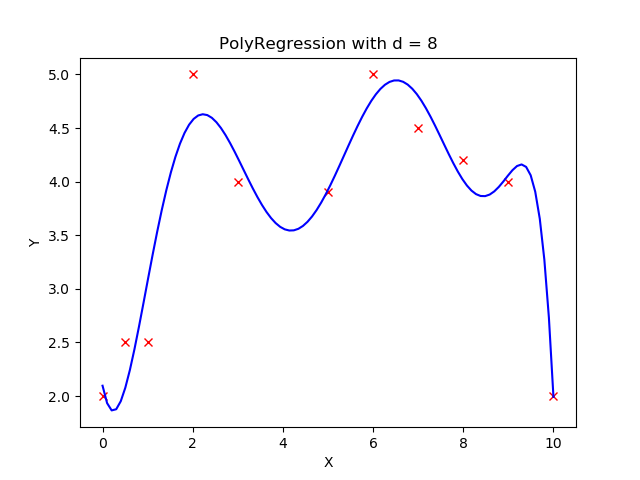
\includegraphics[width=4in]{HW1/HW1_plots/PolyFit.png}
\end{center} 
If we increase the amount of regularization we get the following plot:
\begin{center}
    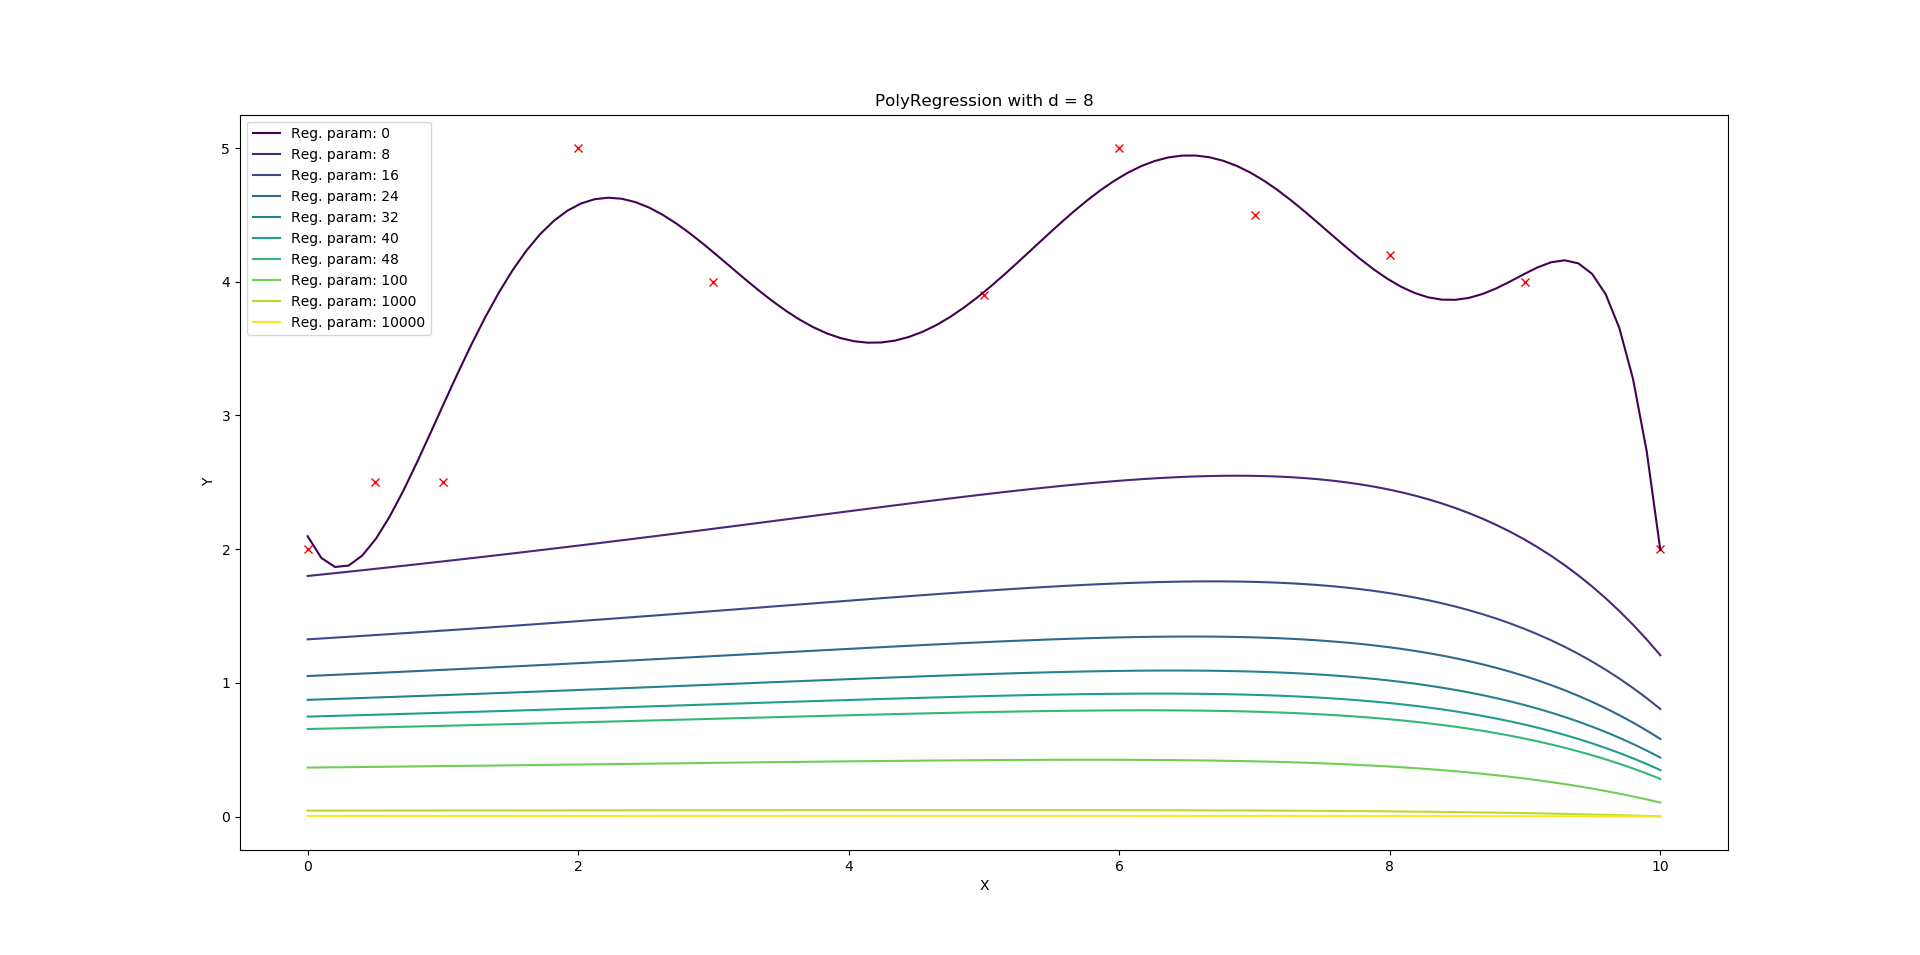
\includegraphics[width=4in]{HW1/HW1_plots/PolyFitRegularization.png}
\end{center} 
Obviously the regularization parameter penalizes large parameter values until the point where said penalty is large enough for the fit to not even deviate from offset value. The implementation of polynomial regression is based on the provided closed form solution:

\newpage
\begin{lstlisting}[language=Python]
import numpy as np

class PolynomialRegression:
    def __init__(self, degree=1, reg_lambda=1E-8):
        """
        Constructor
        """
        self.regLambda = reg_lambda
        self.degree = degree
        self.theta = None
        self._mean = None
        self._std = None

    def _expandToDegree(self, X, degree=None):
        """Expands the given column vector to a (n,d) matrix where elements are
        powers of values x_i including the zero-th order.

        [x1, ... x_n]^T = [[1, x1, x_1^2, ... x_1d^d],
                                       ...
                           [1, x_n, x_n^2, ... x_nd^d]]
        """
        if degree is None:
            degree = self.degree
        return (X[:,None]**np.arange(degree+1))[:, 0, :]

    def polyfeatures(self, X, degree):
        """
        Expands the given X into an n * d array of polynomial features of
        degree d.

        Returns:
            A n-by-d numpy array, with each row comprising of
            X, X * X, X ** 3, ... up to the dth power of X.
            Note that the returned matrix will not include the zero-th power.

        Arguments:
            X is an n-by-1 column numpy array
            degree is a positive integer
        """
        self.degree = degree
        return self._expandToDegree(X, degree)[:, 1:]

    def standardize(self, X, mean=None, std=None):
        """Returns a standardized copy of the array using the given weights.

        Standardization is performed by offsetting by mean and dividing by
        variance on a per column basis.
        """
        mean = self._mean if mean is None else mean
        std = self._std if std is None else std
        standardized = []
        for row in X:
            standardized.append((row-mean)/std)
        return np.vstack(standardized)

    def fit(self, X, y):
        """
            Trains the model
            Arguments:
                X is a n-by-1 array
                y is an n-by-1 array
            Returns:
                No return value
            Note:
                You need to apply polynomial expansion and scaling
                at first
        """
        # expand to polynomial of degree d
        X_ = self.polyfeatures(X, self.degree)

        # standardize the matrix and remember the weights
        self._mean = np.mean(X_, axis=0)
        self._std = np.std(X_, axis=0)
        X_ = self.standardize(X_)

        # add a column of ones
        X_ = np.c_[np.ones([len(X), 1]), X_]

        # construct reg matrix
        reg_matrix = self.regLambda * np.eye(self.degree+1)
        reg_matrix[0,0] = 0

        # analytical solution (X'X + regMatrix)^-1 X' y
        self.theta = np.linalg.pinv(X_.T.dot(X_) + reg_matrix).dot(X_.T).dot(y)
        return self.theta

    def predict(self, X):
        """
        Use the trained model to predict values for each instance in X
        Arguments:
            X is a n-by-1 numpy array
        Returns:
            an n-by-1 numpy array of the predictions
        """
        X_ = self.polyfeatures(X, self.degree)
        X_ = self.standardize(X_)
        X_ = np.c_[np.ones([len(X), 1]), X_]
        return X_.dot(self.theta)
\end{lstlisting} 

\newpage
The code that produces the various regularization parameter plots is a modification of the provided testpolyregunivariate.py script. 

\begin{lstlisting}[language=Python]
import numpy as np
import matplotlib.pyplot as plt
from matplotlib.pyplot import cm
from polyreg import PolynomialRegression

if __name__ == "__main__":
    """Test effects of regularization parameters by plotting
    results of fits with different regularization parameters.
    """
    # pick the polynomial degree and regularization parameters
    d = 8
    reg_lambdas = list(range(0, 50, 8))
    reg_lambdas.extend([100, 1000, 10000])

    # load the data, accidentaly override a python builtin keyword
    filePath = "data/polydata.dat"
    file = open(filePath,'r')
    allData = np.loadtxt(file, delimiter=',')

    # adopt a horrible naming convention
    X = allData[:, [0]]
    y = allData[:, [1]]

    # fit with different regression parameters and store results
    xAxisData, yAxisData = [], []
    for reg_lambda in reg_lambdas:
        model = PolynomialRegression(degree=d, reg_lambda=reg_lambda)
        model.fit(X, y)

        # output predictions
        xpoints = np.linspace(np.max(X), np.min(X), 100).reshape(-1, 1)
        ypoints = model.predict(xpoints)

        xAxisData.append(xpoints)
        yAxisData.append(ypoints)

    # overplot fit results
    colors = cm.viridis(np.linspace(0, 1, len(yAxisData)))
    fig, ax = plt.subplots()
    # points
    ax.plot(X, y, 'rx')
    for x, y, color, label in zip(xAxisData, yAxisData, colors, reg_lambdas):
        ax.plot(x, y, color=color, label=f"Reg. param: {label}")
    ax.set_title('PolyRegression with d = '+str(d))
    ax.set_xlabel('X')
    ax.set_ylabel('Y')
    plt.legend()
    plt.show()
\end{lstlisting} 






\newpage
A.5. \points{10} In this problem we will examine the bias-variance tradeoff through learning curves. Learning curves provide a valuable mechanism for evaluating the bias-variance tradeoff. Implement the learningCurve()function in polyreg.py to compute the learning curves for a given training/test set. The learningCurve(Xtrain,ytrain, Xtest, ytest, degree, regLambda) function should take in the training data (Xtrain,ytrain), the testing data (Xtest,ytest), and values for the polynomial degree $d$ and regularization parameter $\lambda$.The function should return two arrays, errorTrain (the array of training errors) and errorTest(the array of testing errors). The ith index (start from 0) of each array should return the training error (or testing error) for learning with $i+1$ training instances. Note that the 0th index actually won’t matter, since we typically start displaying the learning curves with two or more instances. When computing the learning curves, you should learn on $X_\text{train}[0:i]$ for $i= 1,...,\text{numInstances(Xtrain) + 1}$,each time computing the testing error over the entire test set. There is no need to shuffle the training data, or to average the error over multiple trials - just produce the learning curves for the given training/testing sets with the instances in their given order. Recall that the error for regression problems is given by:
$$\frac{1}{n}\sum_{i=1}^n h_\theta (x_i) - y_i)^2 $$
Once the function is written to compute the learning curves, run thetestpolyreglearningCurve.py script to plot the learning curves for various values of $\lambda$ and $d$.\\
\begin{center}
    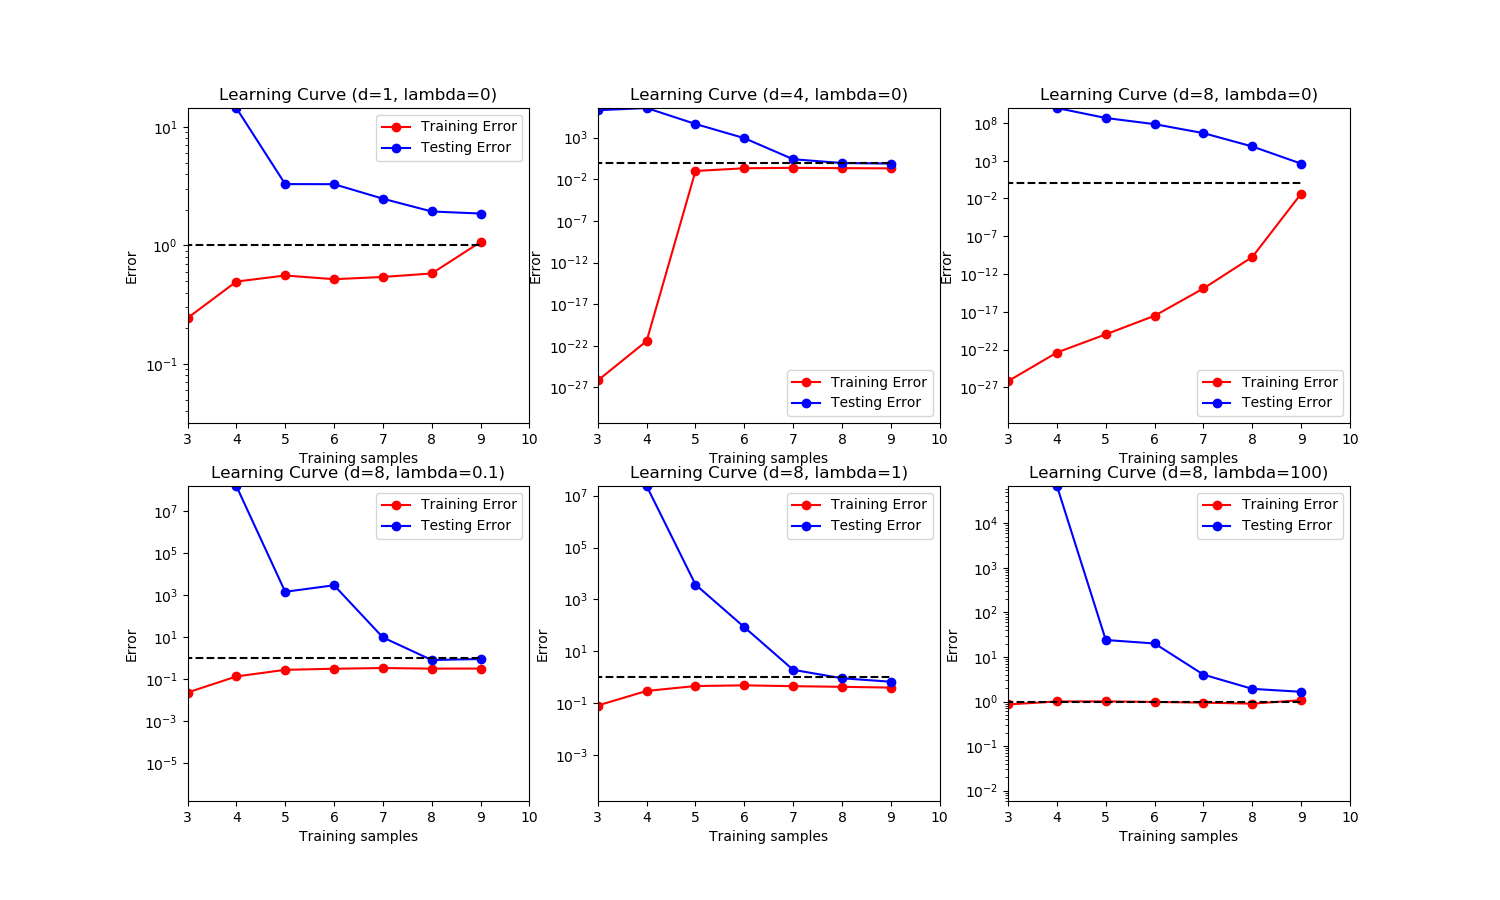
\includegraphics[width=4in]{HW1/HW1_plots/LearningCurves.png}
\end{center} 
\begin{lstlisting}[language=Python]
def learningCurve(Xtrain, Ytrain, Xtest, Ytest, reg_lambda, degree):
    """
    Compute learning curve

    Arguments:
        Xtrain -- Training X, n-by-1 matrix
        Ytrain -- Training y, n-by-1 matrix
        Xtest -- Testing X, m-by-1 matrix
        Ytest -- Testing Y, m-by-1 matrix
        regLambda -- regularization factor
        degree -- polynomial degree

    Returns:
        errorTrain -- errorTrain[i] is the training accuracy using
        model trained by Xtrain[0:(i+1)]
        errorTest -- errorTrain[i] is the testing accuracy using
        model trained by Xtrain[0:(i+1)]

    Note:
        errorTrain[0:1] and errorTest[0:1] won't actually matter, since we start displaying the learning curve at n = 2 (or higher)
    """

    n = len(Xtrain)

    errorTrain = np.zeros(n)
    errorTest = np.zeros(n)

    regressModel = PolynomialRegression(degree=degree, reg_lambda=reg_lambda)

    for i in range(1, n):
        data = Xtrain[0:i+1]
        labels = Ytrain[0:i+1]

        regressModel.fit(data, labels)

        fitTrain = regressModel.predict(data)
        fitTest = regressModel.predict(Xtest)

        errorTrain[i] = 1/len(data) * np.sum((fitTrain-labels)**2)
        errorTest[i] = 1/len(Xtest) * np.sum((fitTest-Ytest)**2)

    return errorTrain, errorTest
\end{lstlisting}




\newpage
\section*{Ridge Regression on MNIST}
A.6. In this problem we will implement a regularized least squares classifier for the MNIST data set. The task is to classify handwritten images of numbers between 0 to 9.You are NOT allowed to use any of the pre-built classifiers in sklearn. Feel free to use any method from numpy or scipy. Remember: if you are inverting a matrix in your code, you are probably doing something wrong (Hint: look at scipy.linalg.solve). Get the data from \url{https://pypi.python.org/pypi/python-mnist}. Load the data as follows:
\begin{lstlisting}[language=Python]
from mnist import MNIST

def load_dataset():
    mndata = MNIST('./data/')
    X_train, labels_train = map(np.array, mndata.load_training())
    X_test, labels_test = map(np.array, mndata.load_testing())
    X_train = X_train/255.0X_test = X_test/255.0
\end{lstlisting}
Each example has features $x_i\in R^d$ (with $d=28\times28=784)$ and label $z_j\in{0,...,9}$. You can visualize a single example $x_i$ with imshow after reshaping it to its original 28x28 image shape (and noting that the label $z_j$ is accurate). We wish to learn a predictor $\hat f$ that takes as input a vector in $R^d$ and outputs an index in ${0,...,9}$. We define our training and testing classification error on a predictor $f$ as:

$$\widehat\epsilon_\text{train} = \frac{1}{N_\text{train}} \sum_{(x,z)\in\text{Training Set}} \1\{f(x)\ne z\}$$
$$\widehat\epsilon_\text{train} = \frac{1}{N_\text{train}} \sum_{(x,z)\in\text{Training Set}} \1\{f(x)\ne z\}$$

We will use one-hot encoding of the labels, i.e. of $(x,z)$ the original label $z\in {0,...,9}$ is mapped to the standard basis vector $e_z$ where $e_z$ is a vector of all zeros except for a $1$ in the $z$th position. We adopt the notation where we have $n$ data points in our training objective with features $x_i\in R^d$ and label one-hot encoded as $y_i\in{0,1}^k$ where in this case $k=10$ since there are 10 digits.
\newpage
\begin{enumerate}
    \item \points{10} In  this  problem  we  will  choose  a  linear  classifier  to  minimize  the  regularized  least  squares objective:
    $$\widehat W = \argmin_{W\in\R^{d\times k}} \sum_{i=0}^n ||W^Tx_i - y_i||^2_2 + \lambda ||W||^2_F$$
    Note that $||W||_F$ corresponds to the Frobenius norm of $W$, i.e. $||W||^2_F = \sum_{j=0}^d\sum_{i=0}^k W^2_{i,j}$. To classify a point $x_i$ we will use the rule $\argmax_{j=0,\hdots 9} e_j^T \widehat W^T x_i$. Note that if $W=[w_1 \hdots w_k]$ then
    \begin{align*}
        \sum_{i=0}^n||W^Tx_i - y_i||^2_2 + \lambda||W||^2_F &= 
        \sum_{j=0}^k\left[ \sum_{i=0}^n(e^T_jW^Tx_i - e_j^Ty_i)^2 + \lambda ||W_{e_j}||^2\right] \\
        &= \sum_{j=0}^k\left[ \sum_{i=0}^n(w_j^Tx_i - e_j^Ty_i)^2 + \lambda ||w_j||^2\right] 
        = \sum_{j=0}^k\left[||Xw_j - Ye_j||^2 + \lambda ||w_j||^2\right]
    \end{align*}{}
    where $X=[x_1\hdots x_n]^T\in\R^{n\times d}$ and $Y=[y_1\hdots y_n]^T\in\R^{n\times k}$. Show that:
    $$\widehat W = (X^TX+\lambda I)^{-1}X^TY$$ \\
    
    In class, lecture 3 slide cca. 25 onward, it was already shown how to decompose $\argmin_W\sum_i^k (||xw_i-y_i||^2+\lambda ||w||^2_2)$ as a $\hat w = (X^TX+\lambda I)^{-1}X^Ty$ when we were trying to derive the closed form solution for least squares problem. This problem is effectively asking us to do the same except it is also required from us to notice that by stacking the data points into a matrix, so that $X=[x_1 \hdots x_N]^T$ and $Y=[y_1 \hdots y_N]^T$\footnote{note however that each $x_i \in \R^d$ and $y_i\in \{0,1\}^k$, thus producing what was given to us in the problem itself $X=[x_1\hdots x_n]^T\in\R^{n\times d}$ and $Y=[y_1\hdots y_n]^T\in\R^{n\times k}$.}, by simple extension we can express the $W$ as an $k\times d$ matrix by stacking the single decomposition as:
    $$ \widehat W = 
    \begin{bmatrix} 
        (X^TX+\lambda I_d)^{-1}X^Ty_1 \\ 
        \vdots \\ 
        (X^TX+\lambda I_d)^{-1}X^Ty_k
    \end{bmatrix} 
    = (X^TXW+\lambda I_d)^{-1}X^TY \in \R^{k\times d}
    $$
    I suspect what is really wanted of us is to take the gradient with respect to $W$ of the given expression for $\widehat W$. Starting from the last line of the hint, keeping in mind $Ye_j=y_j$: 
    \begin{align*}
        &\sum_{j=0}^k \frac{\partial}{\partial w_j} \left(||Xw_j - y_j||^2 + \lambda ||w_j||^2\right) = 0 \\
        &\sum_{j=0}^k 2X^T(Xw_j - y_j) + 2\lambda w_j = 0 \\
        2&\sum_{j=0}^k X^TXw_j - X^Ty_j + \lambda w_j = 0 \\
        &\sum_{j=0}^k (X^TX + \lambda)w_j = \sum_{j=0}^k X^Ty_j \\
        &\sum_{j=0}^k w_j = \sum_{j=0}^k \frac{X^Ty_j}{(X^TX + \lambda)} \\
    \end{align*}{}
    Which is exactly the entire $\widehat W$ if we stack all of the $w_j$ elements on top of each other in a matrix, keeping in mind that the same needs to happen for $y$ and the $w_j$ that was divided out next to $\lambda$:
    $$W = (X^TX+\lambda I_d)^{-1}X^Ty$$
    
    \newpage
    \item \points{10} Code up a function train that takes as input $X\in\R^{n\times d},Y\in {0,1}^{n\times k},\lambda>0$ and returns $\hat W$.
    \begin{enumerate}
        \item Code up a function predict that takes as input $W\in\R^{d\times k},X\in\R^{m\times d}$ and returns an m-length vector with the i-th entry equal to $\argmax_{j=0,...,9}e^T_jW^Tx_i$ where $x_i$ is a column vector representing the i-th example from $X$.
        \item Train $\widehat W$ on the MNIST training data with $\lambda = 10-4$ and make label predictions on the test data. What is the training and testing error? Note that they should both be about 15\%.
    \end{enumerate}
    The full code is below. Running it returns error values:
    
\begin{lstlisting}[language=Bash]
(cse) :~$ python ridge_regression.py 
Train error: 0.14805
Test error: 0.1466
\end{lstlisting}

\begin{lstlisting}[language=Python]
import numpy as np
from scipy import linalg
import matplotlib . pyplot as plt

from mnist import MNIST


def load_mnist_dataset(path="data/mnist_data/"):
    """Loads MNIST data located at path.

    MNIST data are 28x28 pixel large images of letters.

    Parameters
    ----------
    path : `str`
        path to the data directory

    Returns
    -------
    train : `np.array`
        train data normalized to 1
    trainlabels : `np.array`
        train data labels
    test : `np.array`
        test data normalized to 1
    testLabels : `np.array`
        test data labels
    """
    mndata = MNIST("data/mnist_data/")

    train, trainLabels = map(np.array, mndata.load_training())
    test, testLabels  = map(np.array, mndata.load_testing())

    train = train/255.0
    test = test/255.0

    return train, trainLabels, test, testLabels


def one_hot(length, index):
    """Given an index and length k returns an array where all elements are zero
    except the one at index location, where the value is 1.

    Parameters
    ----------
    length : `int`
        Length of the almost-zero array.
    index : `int`
        Index at which element value is set to 1

    Returns
    -------
    arr : `np.array`
        Array of zeros except for arr[index]=1.
    """
    arr = np.zeros(length)
    arr[index] = 1
    return arr


def train(X, Y, lamb):
    """Given data, labels and regularization constant lambda solves

    $$ W = (X^T X) + \lambda I $$

    to retrieve weights of our model.

    Parameters
    ----------
    X : `np.array`
        Data to fit to
    Y : `np.array`
        Data labes, a length 10 array where index of element with value 1 marks
        the number the number respective data point x represents.
    lamb : `float`
        Regularization parameter lambda.

    Returns
    -------
    wHat : `np.array`
        Matrix of weights that minimize the linear least squares.
    """
    n, d = X.shape
    a = np.dot(X.T, X) + lamb*np.eye(d)
    b = np.dot(X.T, Y)
    wHat = linalg.solve(a, b)

    return wHat


def predict(W, data, labelDim):
    """Given weights, data and the dimension of the labels space predicts what
    label is the data most likely representing.

    Parameters
    ----------
    W : `np.array`
        Array of weights of our model.
    data : `np.array`
        Array of data to classify
    labelDim : `int`
        Label space dimension

    Returns
    -------
    classifications : `np.array`
        Array of final predicted classifications of the data.
    """
    predictions = np.dot(data, W)
    # pick out only the most probably values, i.e. the maxima
    maxPredictions = np.argmax(predictions, axis=1)
    classifications = np.array([one_hot(labelDim, y) for y in maxPredictions])
    return classifications


def calc_success_fraction(W, data, labels):
    """Given weights, data and labels predicts the labels of the data and by
    comparing them to the given labels calculates the fraction of the predicted
    classifications that were correct and wrong as a

    fracWrong = (\sum |predicted - actualLabel|) / (2*N_data)
    fracCorrect = 1 - fracWrong

    Parameters
    ----------
    W : `np.array`
        Weights of our model
    data : `np.array`
        data we want to predict labels for
    labels : `np.array`
        labels of actual class the data

    Returns
    -------
    fracCorrect : `float`
        Fraction of correctly predicted labels
    fracWrong : `float`
        Fraction of incorrectly predicted labels
    """
    n, d = data.shape
    labelDim = labels.shape[-1]

    wrong = np.sum(np.abs(predict(W, data, labelDim) - labels)) / 2.0
    # 2 is required because abs value will contribute double to the sum
    fracWrong = wrong/n
    fracCorrect = 1 - fracWrong

    return fracCorrect, fracWrong


def mainA6(lambd=1e-4):
    """Given the dimension of label space and regularization parameter value,
    trains a model on the MNIST train dataset, predicts the labels on the MNIST
    test dataset and calculates the fraction of wrongly predicted labels.

    Parameters
    ----------
    lambd : `float`
        Regularization parameter (lamda)

    Returns
    -------
    trainErr : `float`
        Training error, fraction of incorrectly labeled train data
    testErr : `float`
        Test error, fraction of incorrectly labeled test data
    """
    trainData, trainLabels, testData, testLabels = load_mnist_dataset()
    n, d = trainData.shape
    labelDim = trainLabels.max() + 1 

    trainOneHot = np.array([one_hot(labelDim, y) for y in trainLabels])
    testOneHot  = np.array([one_hot(labelDim, y) for y in testLabels])

    wHat = train(trainData, trainOneHot, lambd)

    trainErr = calc_success_fraction(wHat, trainData, trainOneHot)[-1]
    testErr  = calc_success_fraction(wHat, testData,  testOneHot)[-1]
    print(f"Train error: {trainErr}")
    print(f"Test error: {testErr}")

    return trainErr, testErr


if __name__ == "__main__":
    mainA6()
    #mainB2()
    #plotB2()
    #confidence_intervalB2()

\end{lstlisting}
    
    
    
\end{enumerate}{}



\newpage

\end{document}
